
%\begin{figure}
  \begin{center}
    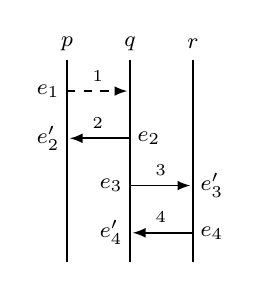
\begin{tikzpicture}[>=stealth,node distance=3.2cm,shorten >=1pt,
      every state/.style={text=black, scale =0.8}, semithick,
      font={\fontsize{8pt}{12}\selectfont}]
	\begin{scope}[xshift = 9cm, scale = 0.8]
		\node at (-0.3, -0.75)  (e)    {$e_1$};
		\node at (1.3, -1.5)  (e)    {$e_2$};
		\node at (-0.3, -1.5)  (e)    {$e_2'$};
		\node at (0.7, -2.25)  (e)    {$e_3$};
		\node at (2.3, -2.25)  (e)    {$e_3'$};
		\node at (2.3, -3)  (e)    {$e_4$};
		\node at (0.7, -3)  (e)    {$e_4'$};
		%MACHINES
		\draw (0,0) node{$p$} ;
		\draw (1,0) node{$q$} ;
		\draw (2,0) node{$r$} ;
		\draw (0,-0.25) -- (0,-3.5) ;
		\draw (1,-0.25) -- (1,-3.5);
		\draw (2, -0.25) -- (2, -3.5) ;
		%MESSAGES
		\draw[>=latex,->, dashed] (0,-0.75) -- (1, -0.75) node[midway,above]{$\amessage_1$};

		\draw[>=latex,->] (1, -1.5) -- (0, -1.5) node[midway, above] {$\amessage_2$};

		\draw[>=latex,->] (1,-2.25) -- (2,-2.25) node[midway, above] {$\amessage_3$};

		\draw[>=latex,->] (2,-3) -- (1,-3) node[midway,above] {$\amessage_4$};
	\end{scope}

\end{tikzpicture}
\captionof{figure}{MSC $\msc_1$}
\label{fig:msc_weak_univer}

\end{center}
%\alain{NIce}
%\end{figure}
